\documentclass[12pt]{beamer}
\usetheme{Madrid}
\usepackage[utf8]{inputenc}
\usepackage[portuguese]{babel}
\usepackage[T1]{fontenc}
\usepackage{amsmath}
\usepackage{amsfonts}
\usepackage{amssymb}
\usepackage{graphicx}
\usepackage{capt-of}
\usepackage{tabularx}
\setbeamertemplate{navigation symbols}{} 
\colorlet{beamer@blendedblue}{green!60!black}
\logo{
\includegraphics[scale=0.03]{uea-new.png}}
\usepackage[backend=biber]{biblatex}
\addbibresource{references.bib}

%------------- CAPA ----------------

\title{BURI}
\subtitle{Sistema Android Embarcado de monitoramento da qualidade do ar residencial}
\author{Adevan Neves Santos \\ Orientador: Prof. Jonathas Silva dos Santos}

\date{30 de julho de 2024}

%------------- CAPA ----------------


\begin{document}
    \maketitle

    \begin{frame}
        \frametitle{Sumário}
        \tableofcontents
    \end{frame}

    \section{Introdução}

    \begin{frame}{Introdução}
         O monóxido de carbono (CO) é um gás incolor, inodor e altamente tóxico para o organismo. O risco de morte por monóxido de carbono em pouco tempo de exposição tem relação com a dificuldade de detecção pelos sentidos humanos e sua ação no processo respiratório. 
    \end{frame}
    
    \begin{frame}{Introdução}
        \begin{figure}
            \centering
            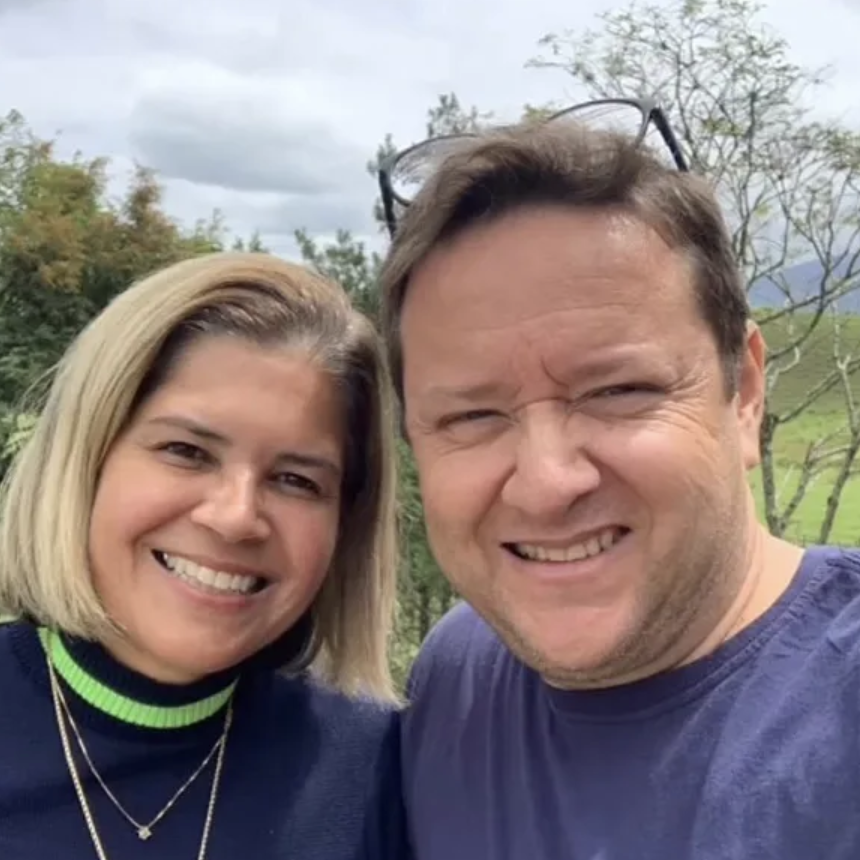
\includegraphics[width=0.50\linewidth]{morte-casal.png}
            \caption{Perícia confirma morte devido CO. Fonte: \cite{morteCO}}
            \label{fig:f1}
        \end{figure}
    \end{frame}

    \section{Objetivo}

    \begin{frame}{Objetivo}
        O objetivo geral é oferecer uma solução de baixo custo em hardware com  ESP32 e sensores para monitorar a qualidade do ar residencial, com ênfase na coleta de dados e alertas  de risco. Os dados coletados serão armazenados e exibidos por meio do aplicativo Android.
    \end{frame}

    \begin{frame}{Objetivo}
        Para atingir o objetivo geral do trabalho, os seguintes objetivos específicos serão cumpridos : 
        \begin{itemize}
            \item Coletar, compreender e tratar as informações dos sensores;
            \item Construir o protótipo do dispositivo embarcado;
            \item Realizar a  comunicação entre o dispositivo e os demais módulos da aplicação;
            \item Desenvolver a API de dados e eventos, assim como a interface do sistema com o usuário;
        \end{itemize}
    \end{frame}

    \section{Metodologia}

    \begin{frame}{Metodologia}
        A metologia aplicada no trabalho basea-se no \textit{embedded design life cycle diagram}, descrito no livro \textit{Embedded Systems Design: An Introduction to Processes, Tools, and  Techniques} \cite{18WorkFlowEmbeddedSystem}. Porém, por ser focado na criação de produtos (e não em pesquisa acadêmica) os seguintes ajustes foram aplicados : fase inicial de pesquisa no domínio do problema e trabalhos relacionados, assim como  escrita da monografia na conclusão do desenvolvimento.
    \end{frame}

    \begin{frame}{Metodologia}
        \begin{figure}
            \centering
            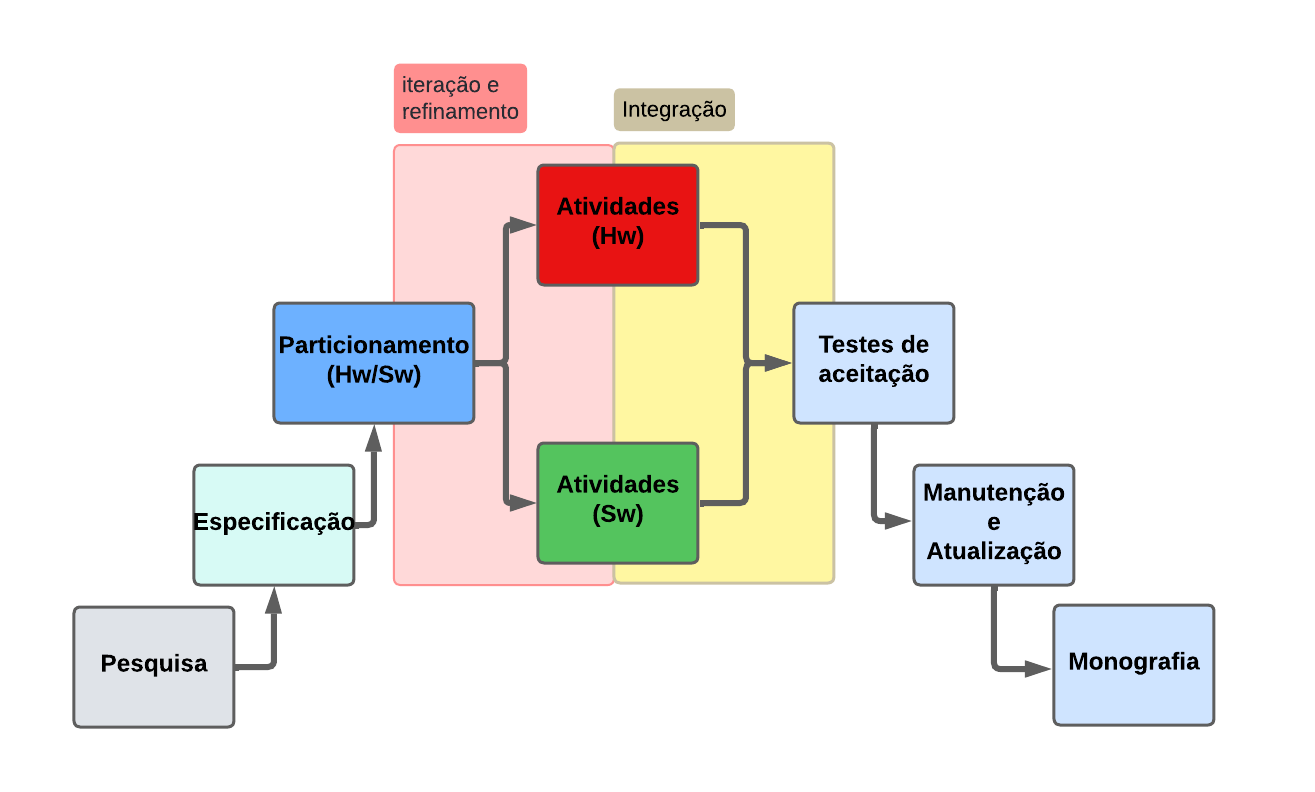
\includegraphics[width=0.97\linewidth]{UEA.png}
            \caption{Fonte: Autoria própria}
            \label{fig:fig2}
        \end{figure}
    \end{frame}

    \section{Contextualização}

    \begin{frame}{Contextualização}
        \begin{itemize}
            \item \textit{Android Open Source Project} (AOSP);
            \item \textit{Internet Of Things} (Iot);
            \item Qualidade do Ar;
        \end{itemize}
    \end{frame}

    \begin{frame}{AOSP}
        O Android é um Sistema Operacional de código aberto baseado na kernel do Linux, focado em dispositivos móveis, cujo projeto é liderado pela empresa Google. Já o \textit{Android Open Source Project} (AOSP) é o projeto  de código aberto com informações e ferramentas necessárias para a implementação de personalizações no Android \cite{aosp-documentation}. 
    \end{frame}

    \begin{frame}{AOSP : Impacto do Android no Brasil}
        \begin{figure}
            \centering
            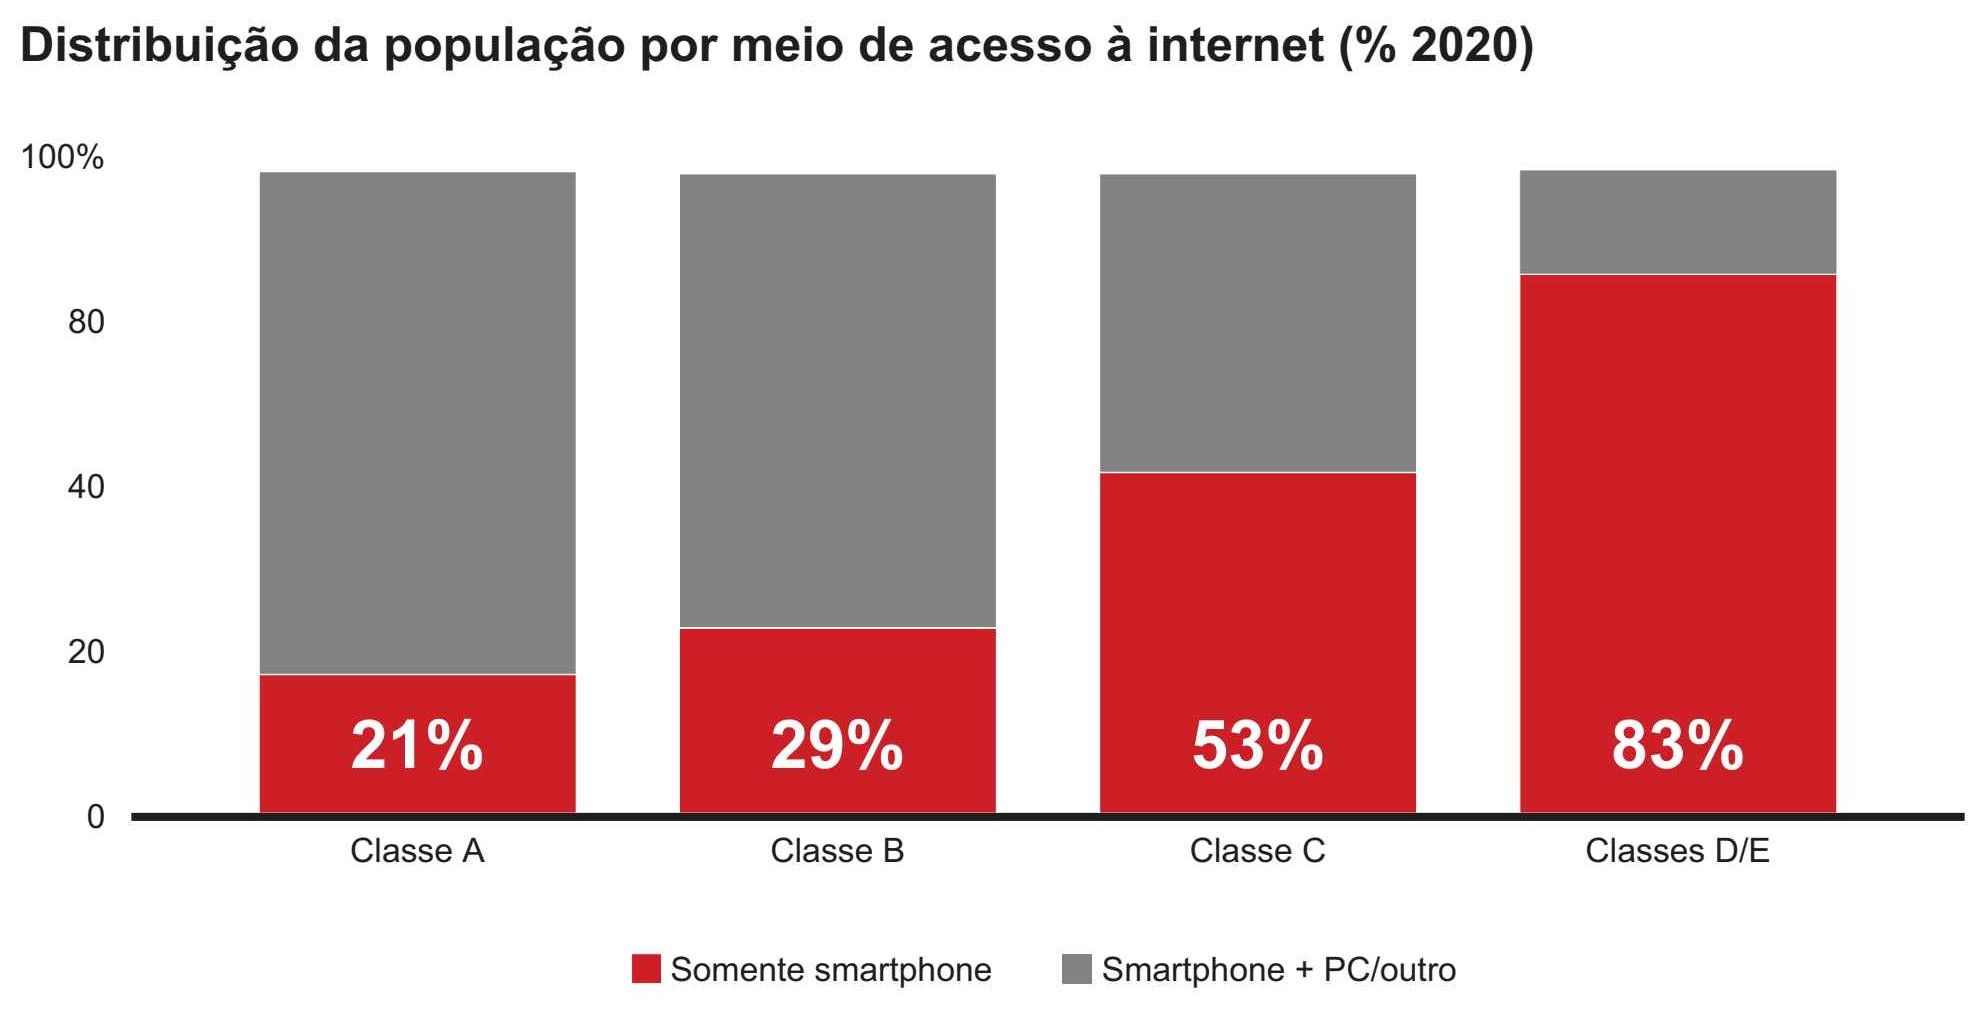
\includegraphics[width=0.92\linewidth]{android-2.png}
            \caption{Fonte: \cite{impactoAndroidBrazil}}
            \label{fig:fig4}
        \end{figure}
    \end{frame}

    \begin{frame}{IOT}
        \textit{Internet of Things} foi o termo utilizado primeiramente em 1999 pelo então pesquisador do \textit{Massachusetts Institute of Technology} (MIT) Kevin Asthon em uma apresentação na Procter \& Gamble (P\&G) sobre a tecnologia do \textit{Radio Frequency Identification} (RFID). Esse conceito tem relação com a comunicação entre dispositivos por meio da internet, assim como a coleta e análise de dados para a tomada de decisões inteligentes \cite{refTermoIOT}.
    \end{frame}

    \begin{frame}{IOT}
        \begin{figure}
            \centering
            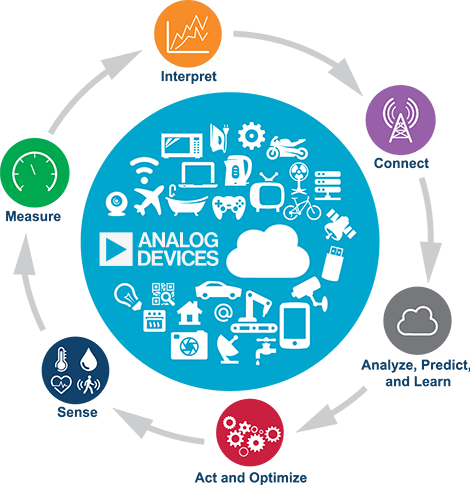
\includegraphics[width=0.5\linewidth]{cicloIOT.png}
            \caption{Fonte: \cite{cicloIOT}}
            \label{fig:fig6}
        \end{figure}
    \end{frame}
    
    \begin{frame}{Qualidade do Ar}
        \begin{figure}
            \centering
            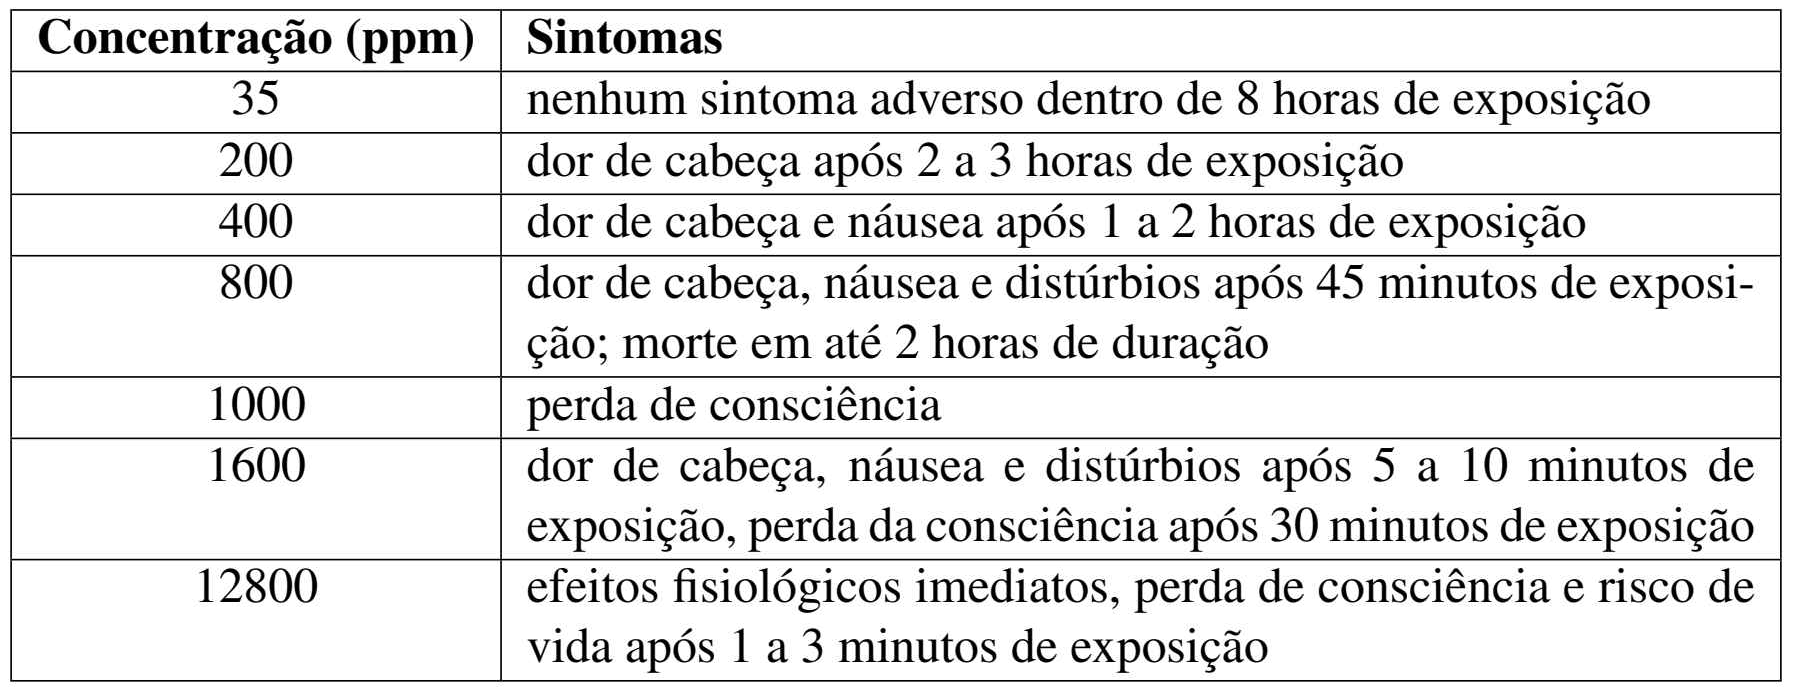
\includegraphics[width=0.95\linewidth]{tabela-co.png}
            \caption{Sintomas de envenenamento por CO baseados na concentração do ar. Fonte: Retirado de \cite{tabelaCO}.}
            \label{fig:f7}
        \end{figure}
    \end{frame}

    \section{Resultados Parciais}

    \begin{frame}{Resultados Parciais}
        \begin{enumerate}
            \item Pesquisa bibliográfica (Etapa 1);
            \item Pesquisa com Questionário (Etapa 2);
        \end{enumerate}
    \end{frame}

    \begin{frame}{Resultados Parciais: Pesquisa}
        Na pesquisa bibliográfica, identificamos trabalhos relacionados no estudo do tema. Portanto, os resultados da etapa foram os seguintes :
        \begin{itemize}
            \item Sumaúma: Estação de monitoramento de plantas domésticas utilizando Android Embarcado e ESP32 \cite{12-UFAM-Sumauma};
            \item Desenvolvimento de um protótipo de dispositivo de baixo custo baseado em Iot (internet of things) para detecção e prevenção de incêndios em ambientes residenciais \cite{11-UEA-IOT-Prev-Inc};
            \item Asfixiantes bioquímicos: Monóxido de carbono y Cianuro \cite{hernandez2022asfixiantes};
        \end{itemize}
    \end{frame}

    \begin{frame}{Resultados Parciais: Questionário}
        Para a fase de especificação do produto, foi produzido um questionário. A pesquisa possui abordagem qualitativa e natureza aplicada, pois o objetivo é entender o problema e elaborar uma proposta de solução. 
    \end{frame}

    \begin{frame}{Resultados Parciais: Questionário}
        \begin{figure}
            \centering
            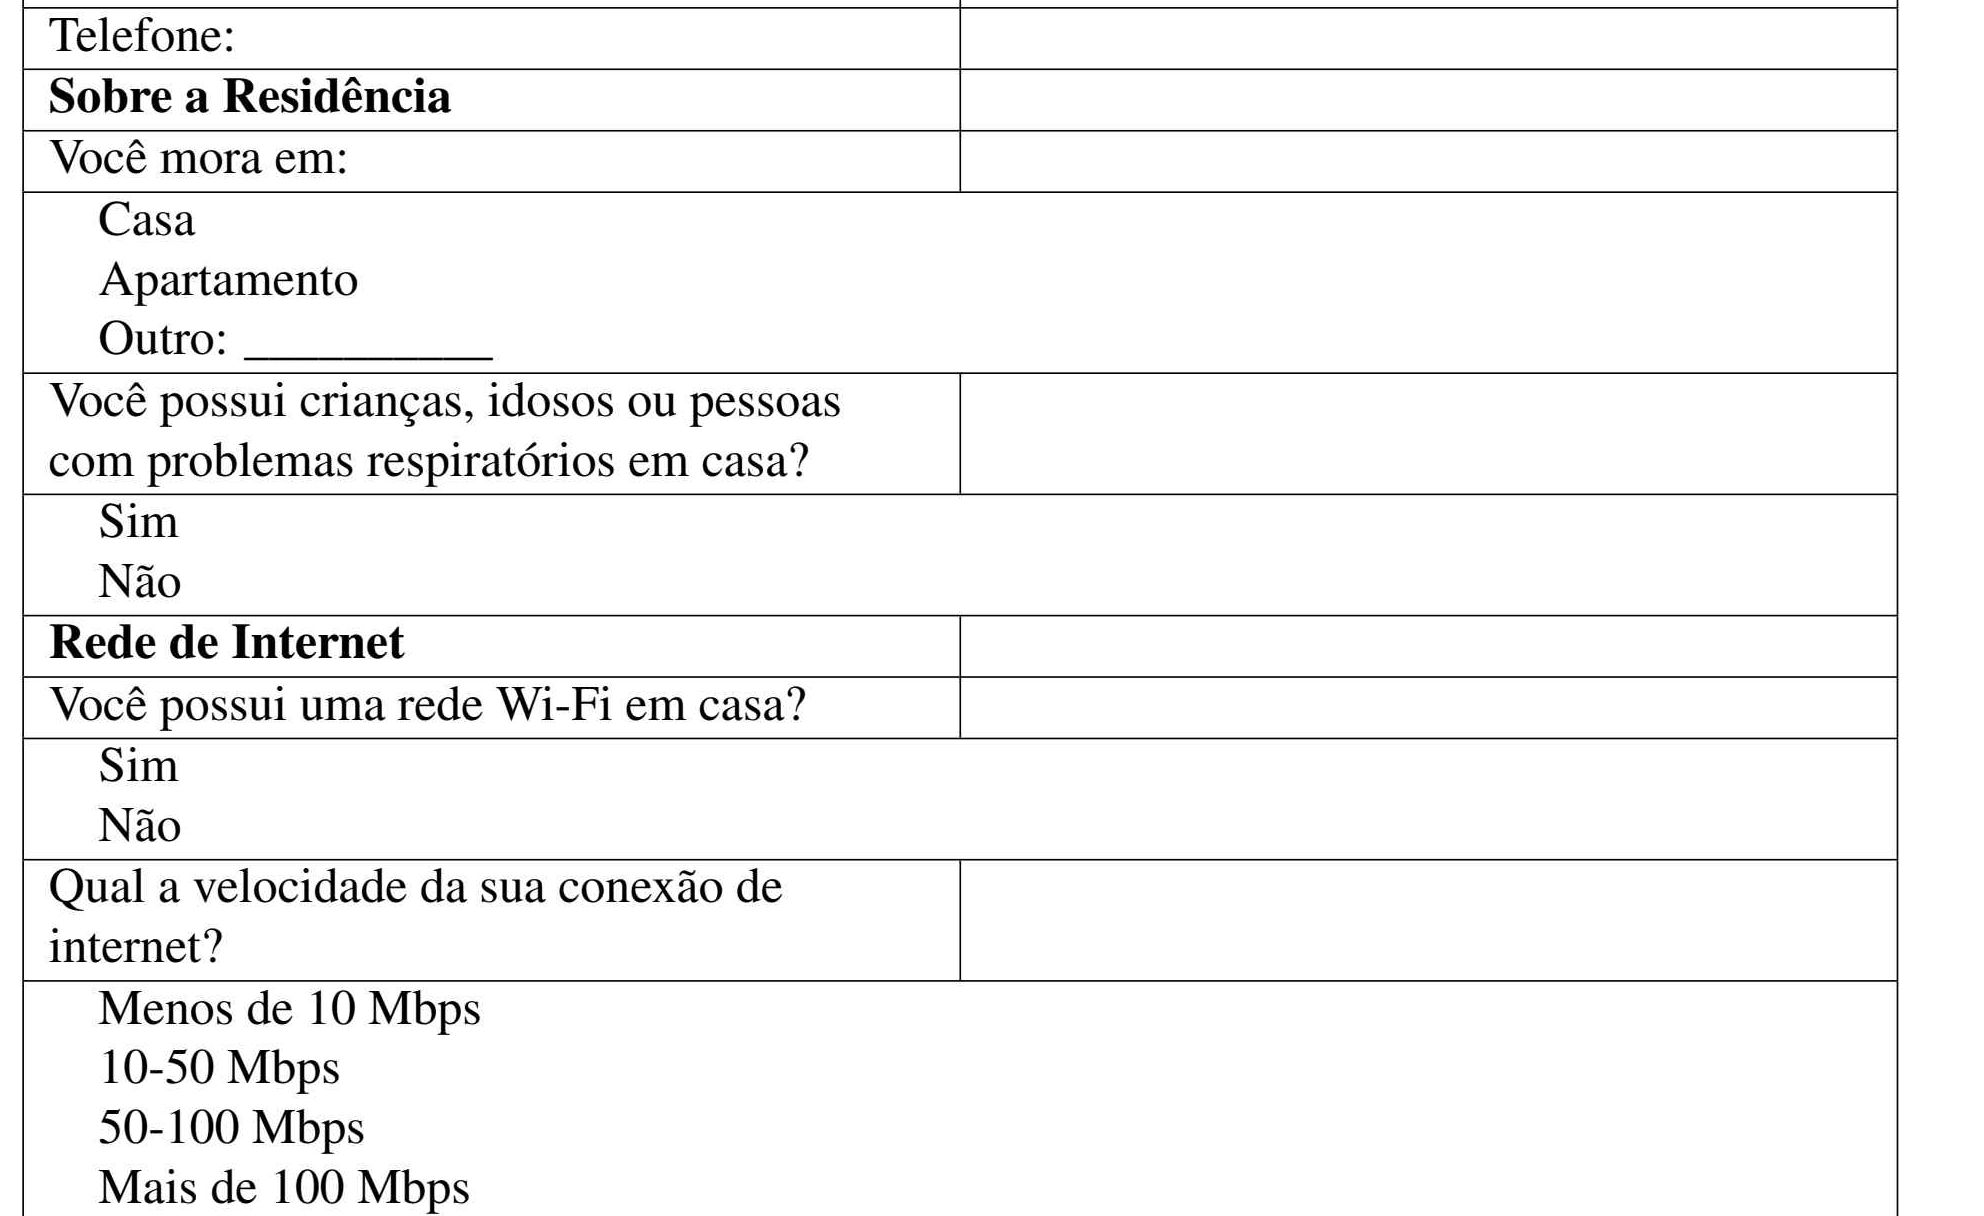
\includegraphics[width=0.8\linewidth]{quest (1).png}
            \caption{Questionário para visitas aos clientes}
            \label{fig:enter-label}
        \end{figure}
    \end{frame}

    \begin{frame}{Resultados Parciais: Montagem do protótipo}
        \begin{figure}
            \centering
            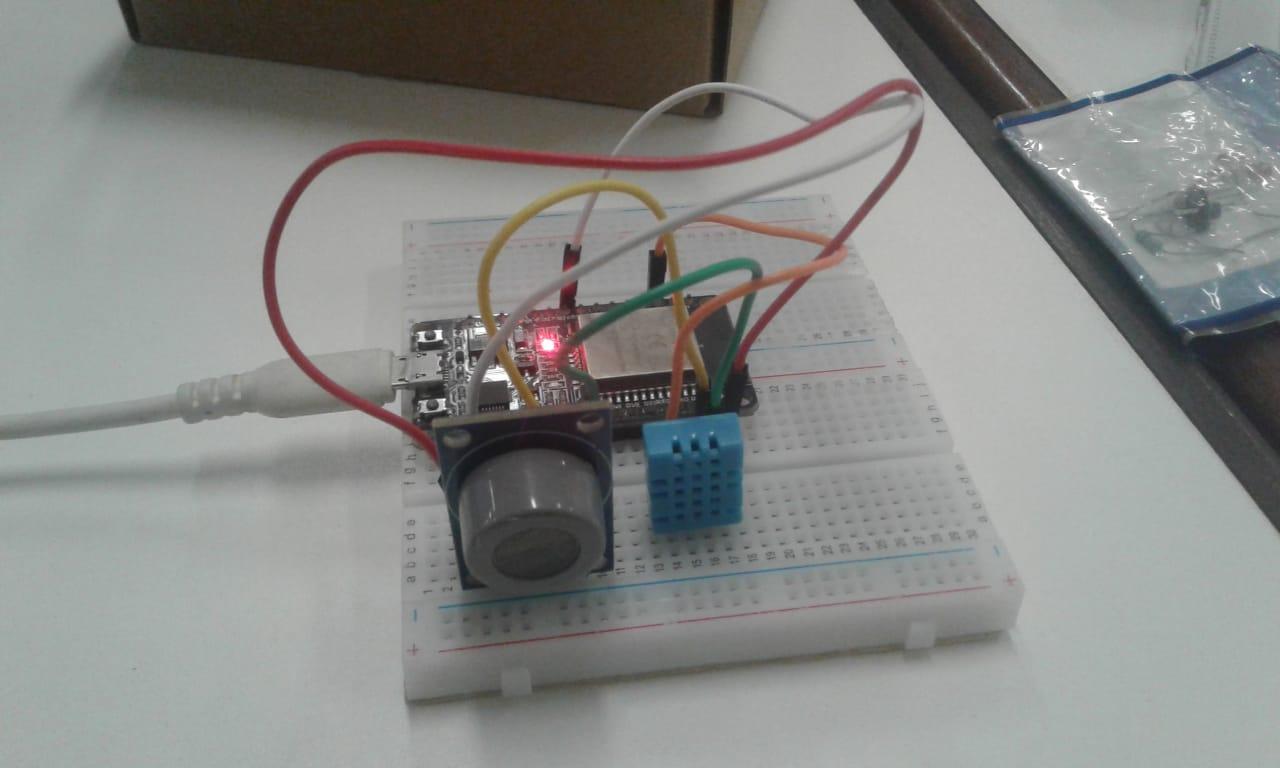
\includegraphics[width=0.7\linewidth]{prototipo.jpeg}
            \caption{Protótipo do Hardware. Fonte : Autoria própria}
            \label{fig:enter-label}
        \end{figure}
    \end{frame}

    \section{Cronograma}

    \begin{frame}{Cronograma}
            \begin{figure}
            \centering
            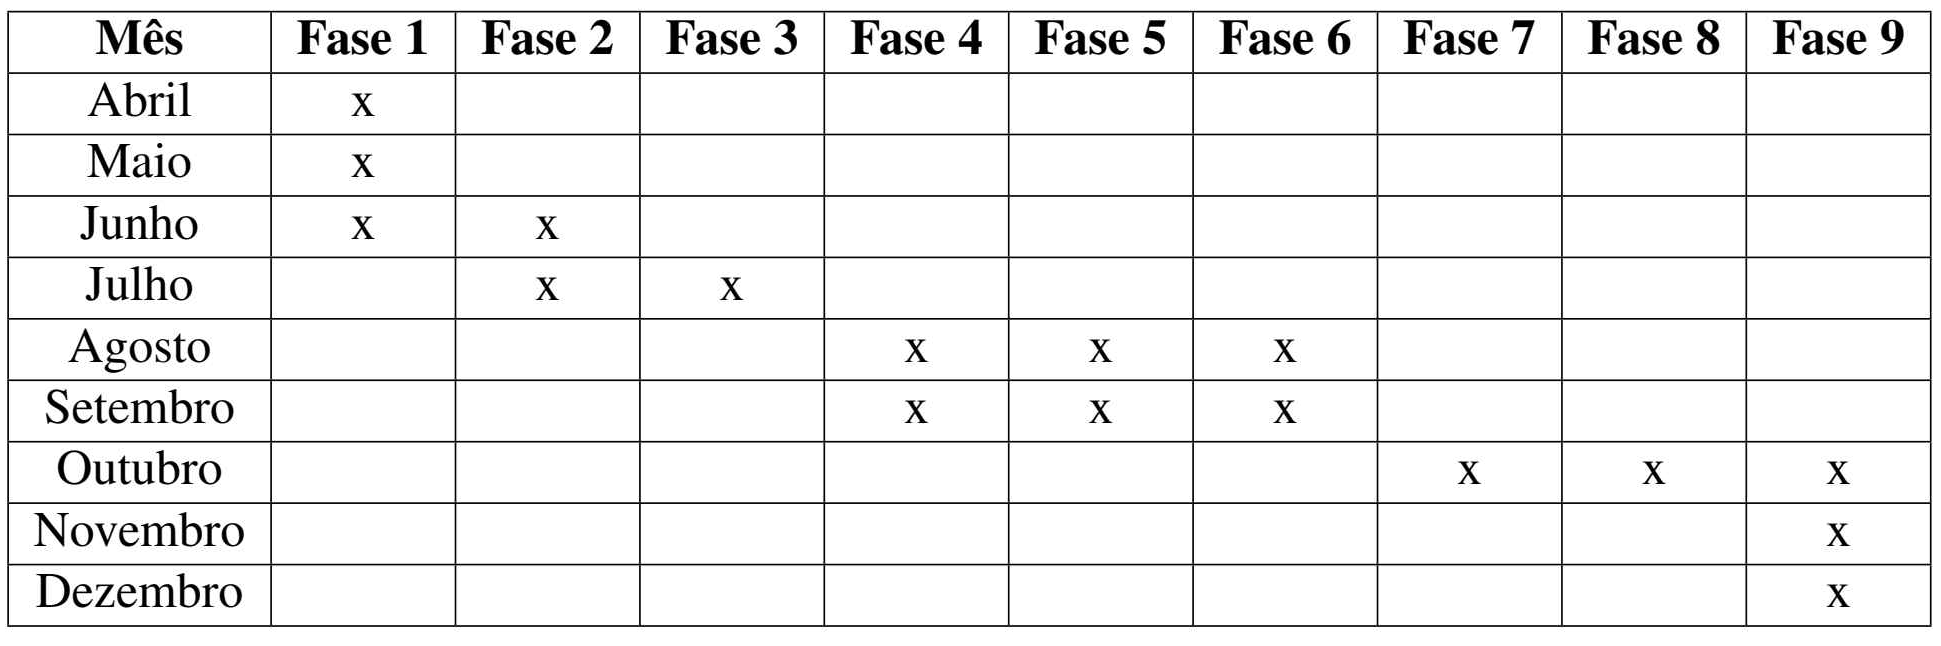
\includegraphics[width=0.95\linewidth]{cronograma.png}
            \caption{Cronograma}
            \label{fig:enter-label}
        \end{figure}
    \end{frame}

    \section{Referências}
    
    \printbibliography
\end{document}